\documentclass[border=1.5pt]{standalone}
\usepackage{amsmath,amssymb}
\usepackage{tikz}
\usetikzlibrary{arrows.meta,calc,positioning,shapes,shapes.misc,shapes.geometric,backgrounds,fit,decorations.pathreplacing,quantikz2}
% Shared colors and styles for the XYZ^2 figures.
% Pauli types: bright tones for fills and bands, deep (800) shades of the same hues for labels.
% The label shades keep the hue of each Pauli, are well separated from each other (CIEDE2000 > 20)
% and have a contrast ratio of at least 2.9 on the coral cells and 4.5 on the sunflower cells.
\definecolor{PauliX}{HTML}{F97316}
\definecolor{PauliY}{HTML}{EC4899}
\definecolor{PauliZ}{HTML}{9333EA}
\definecolor{PauliXText}{HTML}{AC340B}
\definecolor{PauliYText}{HTML}{9D174D}
\definecolor{PauliZText}{HTML}{5B21B6}
% Generator classes: S0 (class B, even links, coral) and gauge (class A, odd links, sunflower)
\definecolor{Szero}{HTML}{F0435E}
\definecolor{SzeroText}{HTML}{BE123C}
\definecolor{Gauge}{HTML}{F59E0B}
\definecolor{GaugeText}{HTML}{B45309}
\colorlet{GaugeGray}{Gauge}
\definecolor{ClassB}{HTML}{FF8A99}
\definecolor{ClassA}{HTML}{FFD23F}
% Logical operators (X-bar violet, Z-bar crimson), errors, ink
\definecolor{LogicalZ}{HTML}{E11D48}
\definecolor{LogicalGold}{HTML}{7C3AED}
\definecolor{ErrRed}{HTML}{1C1917}
\definecolor{InkDark}{HTML}{292524}
\definecolor{InkSoft}{HTML}{57534E}
% Labels drawn on top of colored cells
\colorlet{CellText}{InkDark}
% Noise channels
\definecolor{ErrFlip}{HTML}{EF4444}
\definecolor{Idle}{HTML}{EC4899}
\definecolor{TwoQ}{HTML}{7C3AED}
% Protocol steps
\definecolor{StepPrep}{HTML}{F97316}
\definecolor{StepMeas}{HTML}{D946EF}
\definecolor{StepDec}{HTML}{7C3AED}
\definecolor{StepRec}{HTML}{DB2777}
\tikzset{
  qb/.style={circle, draw=InkDark, line width=0.6pt, fill=white,
             minimum size=4.2mm, inner sep=0pt, font=\scriptsize},
  qbsmall/.style={circle, draw=InkDark, line width=0.5pt, fill=white,
             minimum size=2.6mm, inner sep=0pt},
  hexedge/.style={line width=0.65pt, draw=InkSoft},
  linkedge/.style={line width=1.6pt, draw=InkDark},
  bndedge/.style={line width=0.65pt, draw=InkSoft, densely dashed},
  plabel/.style={font=\scriptsize\bfseries, inner sep=1pt},
  panel/.style={font=\small\bfseries, anchor=north west},
}

\providecommand{\ket}[1]{\left|#1\right\rangle}

\begin{document}
\setlength{\tabcolsep}{0pt}
\begin{tabular}{@{}l@{\hspace{6mm}}l@{}}
\textbf{(a)} & \textbf{(b)}\\[-2pt]
\raisebox{-0.5\height}{%
\begin{quantikz}[row sep={0.95cm,between origins}, column sep=0.2cm]
\lstick{\footnotesize data $u$} & \gate[style={fill=PauliX!30, draw=PauliX}]{R_{b_u}} & \gate[style={fill=ErrFlip!26, draw=ErrFlip}]{\mathcal{F}^{Q_{b_u}}_{p_{\rm r}}} & \gate[style={fill=Idle!26, draw=Idle}]{\mathcal{D}_{p_{\rm i}}} \slice[style={draw=InkSoft, dash pattern=on 2pt off 1.5pt, line width=0.45pt}, label style={text=InkSoft}]{\scriptsize reset} & \targ{} & \gate[2, style={fill=TwoQ!26, draw=TwoQ}]{\mathcal{D}^{(2)}_{p_2}} \slice[style={draw=InkSoft, dash pattern=on 2pt off 1.5pt, line width=0.45pt}, label style={text=InkSoft}]{\scriptsize layer 1} &  & \gate[style={fill=Idle!26, draw=Idle}]{\mathcal{D}_{p_{\rm i}}} \slice[style={draw=InkSoft, dash pattern=on 2pt off 1.5pt, line width=0.45pt}, label style={text=InkSoft}]{\scriptsize layer 2} &  & \gate[style={fill=Idle!26, draw=Idle}]{\mathcal{D}_{p_{\rm i}}} \slice[style={draw=InkSoft, dash pattern=on 2pt off 1.5pt, line width=0.45pt}, label style={text=InkSoft}]{\scriptsize measure} & \ \cdots\  & \gate[style={fill=ErrFlip!26, draw=ErrFlip}]{\mathcal{F}^{Q_{b_u}}_{p_{\rm m}}} & \meter[style={fill=PauliZ!28, draw=PauliZ}]{b_u} \\
\lstick{\footnotesize ancilla} & \gate[style={fill=PauliX!30, draw=PauliX}]{R_{\textcolor{PauliXText}{\boldsymbol{X}}}} & \gate[style={fill=ErrFlip!26, draw=ErrFlip}]{\mathcal{F}^{\textcolor{PauliZText}{\boldsymbol{Z}}}_{p_{\rm r}}} &  & \ctrl{-1} &  & \ctrl{1} & \gate[2, style={fill=TwoQ!26, draw=TwoQ}]{\mathcal{D}^{(2)}_{p_2}} & \gate[style={fill=ErrFlip!26, draw=ErrFlip}]{\mathcal{F}^{\textcolor{PauliZText}{\boldsymbol{Z}}}_{p_{\rm m}}} & \gate[style={fill=PauliZ!28, draw=PauliZ}]{M_{\textcolor{PauliXText}{\boldsymbol{X}}}} & \setwiretype{n} &  &  \\
\lstick{\footnotesize data $l$} & \gate[style={fill=PauliX!30, draw=PauliX}]{R_{b_l}} & \gate[style={fill=ErrFlip!26, draw=ErrFlip}]{\mathcal{F}^{Q_{b_l}}_{p_{\rm r}}} & \gate[style={fill=Idle!26, draw=Idle}]{\mathcal{D}_{p_{\rm i}}} &  & \gate[style={fill=Idle!26, draw=Idle}]{\mathcal{D}_{p_{\rm i}}} & \targ{} &  &  & \gate[style={fill=Idle!26, draw=Idle}]{\mathcal{D}_{p_{\rm i}}} & \ \cdots\  & \gate[style={fill=ErrFlip!26, draw=ErrFlip}]{\mathcal{F}^{Q_{b_l}}_{p_{\rm m}}} & \meter[style={fill=PauliZ!28, draw=PauliZ}]{b_l}
\end{quantikz}}
&
\raisebox{-0.5\height}{%
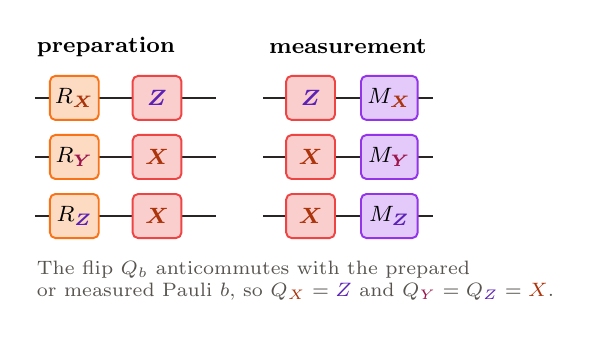
\begin{tikzpicture}[
  op/.style={draw=#1, fill=#1!26, line width=0.7pt, rounded corners=0.7mm, minimum height=0.56cm, minimum width=0.62cm, font=\footnotesize, inner sep=1.5pt},
  wl/.style={line width=0.6pt, draw=InkDark},
]
\node[font=\footnotesize\bfseries, anchor=west] at (-0.1,1.75) {preparation};
\node[font=\footnotesize\bfseries, anchor=west] at (2.85,1.75) {measurement};
\foreach \y/\b/\f in {1.1/X/Z, 0.35/Y/X, -0.4/Z/X}{
  \draw[wl] (0,\y) -- (2.3,\y);
  \node[op=PauliX] at (0.5,\y) {$R_{\textcolor{Pauli\b Text}{\boldsymbol{\b}}}$};
  \node[op=ErrFlip] at (1.55,\y) {$\textcolor{Pauli\f Text}{\boldsymbol{\f}}$};
  \draw[wl] (2.9,\y) -- (5.05,\y);
  \node[op=ErrFlip] at (3.5,\y) {$\textcolor{Pauli\f Text}{\boldsymbol{\f}}$};
  \node[op=PauliZ, minimum width=0.72cm] at (4.5,\y) {$M_{\textcolor{Pauli\b Text}{\boldsymbol{\b}}}$};
}
\node[font=\scriptsize, text=InkSoft, align=left, anchor=north west] at (-0.1,-0.85) {The flip $Q_b$ anticommutes with the prepared\\ or measured Pauli $b$, so $Q_{\textcolor{PauliXText}{X}}=\textcolor{PauliZText}{Z}$ and $Q_{\textcolor{PauliYText}{Y}}=Q_{\textcolor{PauliZText}{Z}}=\textcolor{PauliXText}{X}$.};
\end{tikzpicture}}
\end{tabular}

\end{document}
